% =============================================================================
%  fig_two_pass_estimator.tex
%  Two-pass inverse estimation strategy — timeline + window diagram
% =============================================================================
\documentclass[tikz, border=8pt]{standalone}
\usepackage{tikz}
\usepackage{amsmath}
\usetikzlibrary{arrows.meta, positioning, calc, decorations.pathreplacing,
                patterns, backgrounds}

\definecolor{p1C}  {RGB}{31,  119, 180}
\definecolor{p2C}  {RGB}{214,  39,  40}
\definecolor{fltC} {RGB}{255, 127,  14}

\tikzset{
  tbar/.style = {line width=1.0pt, color=#1},
  arr/.style  = {-{Stealth[length=4.5pt]}, line width=0.85pt},
  brace/.style= {decorate, decoration={brace, amplitude=6pt, raise=3pt},
                 line width=0.8pt},
  lbl/.style  = {font=\footnotesize, align=center},
  ann/.style  = {font=\scriptsize, align=center, color=gray!70!black},
}

\begin{document}
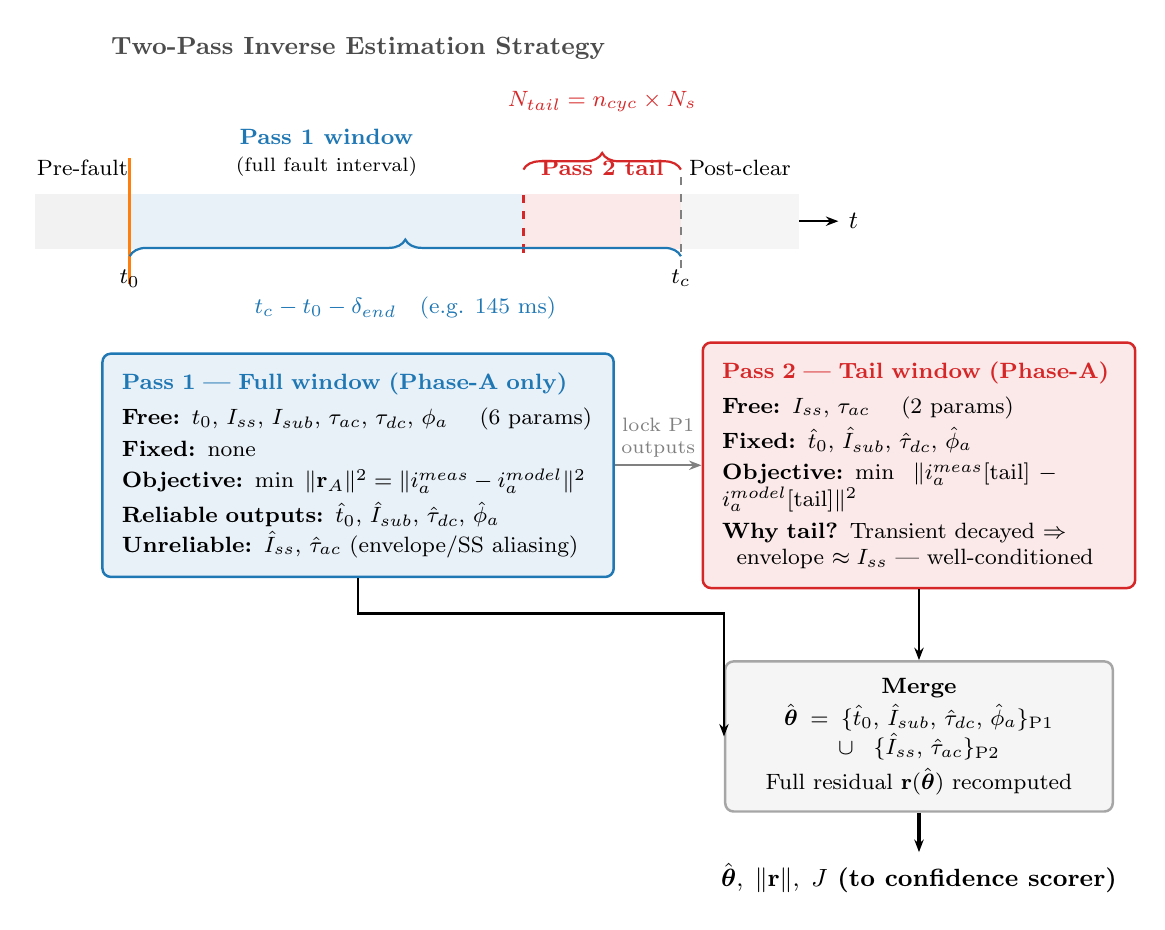
\begin{tikzpicture}

% ============================================================
%  Top section: timeline diagram
% ============================================================

\def\tpre{1.2}   % pre-fault length (cm)
\def\twin{7.0}   % fault window length (cm)
\def\ttail{2.0}  % tail window length (cm)
\def\tpost{1.5}  % post-clear region (cm)

% Time axis
\draw[arr] (0,0) -- ({\tpre+\twin+\tpost+0.5}, 0)
  node[right, font=\small] {$t$};

% --- Region fills ---
\fill[gray!10] (0, -0.35) rectangle (\tpre, 0.35);
\fill[p1C!10]  (\tpre, -0.35) rectangle ({\tpre+\twin}, 0.35);
\fill[p2C!10]  ({\tpre+\twin-\ttail}, -0.35)
               rectangle ({\tpre+\twin}, 0.35);
\fill[gray!8]  ({\tpre+\twin}, -0.35) rectangle ({\tpre+\twin+\tpost}, 0.35);

% --- Boundary lines ---
\draw[tbar=gray,  dashed] (\tpre, -0.6) -- (\tpre, 0.6);
\draw[tbar=fltC,  line width=1.2pt] (\tpre, -0.8) -- (\tpre, 0.8);
\draw[tbar=gray,  dashed] ({\tpre+\twin}, -0.6) -- ({\tpre+\twin}, 0.6);
\draw[tbar=p2C,   dashed] ({\tpre+\twin-\ttail}, -0.4) --
                           ({\tpre+\twin-\ttail}, 0.4);

% --- Labels on timeline ---
\node[lbl, above=0.45cm] at (\tpre/2, 0)       {Pre-fault};
\node[lbl, below=0.5cm]  at (\tpre, 0)          {$t_0$};
\node[lbl, above=0.45cm] at ({\tpre+\twin/2-\ttail/2}, 0)
  {\textcolor{p1C}{\textbf{Pass 1 window}} \\ \scriptsize (full fault interval)};
% Pass 2 tail label — above the strip, between strip top and N_tail brace
\node[lbl] at ({\tpre+\twin-\ttail/2}, 0.68)
  {\textcolor{p2C}{\textbf{Pass 2 tail}}};
\node[lbl, below=0.5cm]  at ({\tpre+\twin}, 0)  {$t_c$};
\node[lbl, above=0.45cm] at ({\tpre+\twin+\tpost/2}, 0)
  {Post-clear};

% Braces
\draw[brace, color=p1C]
  (\tpre, -0.55) -- ({\tpre+\twin}, -0.55)
  node[midway, below=8pt, lbl, color=p1C]
  {$t_c - t_0 - \delta_{end}$\quad (e.g. 145 ms)};

\draw[brace, color=p2C]
  ({\tpre+\twin-\ttail}, 0.55) -- ({\tpre+\twin}, 0.55)
  node[midway, above=20pt, lbl, color=p2C]
  {$N_{tail} = n_{cyc} \times N_s$};

% ============================================================
%  Bottom section: two-pass box diagram
% ============================================================

\def\bY{-2.5}   % baseline y for boxes

% Pass 1 box
\node[rectangle, rounded corners=3pt, draw=p1C, fill=p1C!10, line width=0.9pt,
      text width=6.0cm, align=left, font=\footnotesize, inner sep=7pt]
  (p1box) at ({(\tpre+\twin)/2}, {\bY-0.6})
{
  \textbf{\textcolor{p1C}{Pass 1 — Full window (Phase-A only)}}\\[3pt]
  \textbf{Free:} $t_0,\,I_{ss},\,I_{sub},\,\tau_{ac},\,\tau_{dc},\,\phi_a$ \quad (6 params)\\[2pt]
  \textbf{Fixed:} none\\[2pt]
  \textbf{Objective:} $\min\;\|\mathbf{r}_A\|^2 = \|i_a^{meas} - i_a^{model}\|^2$\\[2pt]
  \textbf{Reliable outputs:} $\hat{t}_0,\,\hat{I}_{sub},\,\hat{\tau}_{dc},\,\hat{\phi}_a$\\[1pt]
  \textbf{Unreliable:} $\hat{I}_{ss},\,\hat{\tau}_{ac}$ (envelope/SS aliasing)
};

% Arrow Pass1 → Pass2 — plain arrow, label above outside both boxes
\draw[arr, color=gray] (p1box.east) -- ++(1.1, 0);
\node[font=\scriptsize, color=gray, align=center]
  at ($(p1box.east) + (0.55, 0.35)$)
  {lock P1\\outputs};

% Pass 2 box
\node[rectangle, rounded corners=3pt, draw=p2C, fill=p2C!10, line width=0.9pt,
      text width=5.0cm, align=left, font=\footnotesize, inner sep=7pt,
      right=1.1cm of p1box]
  (p2box)
{
  \textbf{\textcolor{p2C}{Pass 2 — Tail window (Phase-A)}}\\[3pt]
  \textbf{Free:} $I_{ss},\,\tau_{ac}$ \quad (2 params)\\[2pt]
  \textbf{Fixed:} $\hat{t}_0,\,\hat{I}_{sub},\,\hat{\tau}_{dc},\,\hat{\phi}_a$\\[2pt]
  \textbf{Objective:}
  $\min\;\|i_a^{meas}[\text{tail}] - i_a^{model}[\text{tail}]\|^2$\\[2pt]
  \textbf{Why tail?} Transient decayed $\Rightarrow$\\
  $\;$ envelope $\approx I_{ss}$ — well-conditioned
};

% Merge box
\node[rectangle, rounded corners=3pt, draw=gray!70, fill=gray!8, line width=0.9pt,
      text width=4.5cm, align=center, font=\footnotesize, inner sep=6pt,
      below=0.9cm of p2box]
  (merge)
{
  \textbf{Merge}\\[2pt]
  $\hat{\boldsymbol{\theta}} = \{\hat{t}_0,\,\hat{I}_{sub},\,\hat{\tau}_{dc},\,\hat{\phi}_a\}_{\text{P1}}$\\
  $\cup\;\{\hat{I}_{ss},\,\hat{\tau}_{ac}\}_{\text{P2}}$\\[2pt]
  Full residual $\mathbf{r}(\hat{\boldsymbol{\theta}})$ recomputed
};

\draw[arr] (p2box.south) -- (merge.north);
\draw[arr] (p1box.south) -- ++(0,-0.45) -| (merge.west);

% Output arrow
\draw[arr, line width=1.1pt]
  (merge.south) -- ++(0,-0.5)
  node[below, font=\small\bfseries]
  {$\hat{\boldsymbol{\theta}},\;\|\mathbf{r}\|,\;J$  (to confidence scorer)};

% ---- Caption label — above the upper brace, clear of timeline labels --------
\node[font=\small\bfseries, color=black!70] at ({(\tpre+\twin)/2}, {2.2})
  {Two-Pass Inverse Estimation Strategy};

\end{tikzpicture}
\end{document}
